\documentclass[12pt,letter]{article}
\usepackage{mathptmx} % added for time new roman font
\usepackage[left=1in,right=1in,top=1in,bottom=1in]{geometry}
\usepackage[latin1]{inputenc}
\usepackage{amsmath}
\usepackage[final]{pdfpages}
\usepackage{caption}	% added for \captionof
\usepackage[textsize=tiny]{todonotes}

% defines all example enviorment
\usepackage[framemethod=tikz]{mdframed} % added for the box around examples
\newtheorem{ex}{Example}
\numberwithin{ex}{section} % allows for the use of example numbers that lign up with the section numbers
\newenvironment{example}{\begin{mdframed}[middlelinewidth=0.5mm]\begin{ex}\normalfont}{\end{ex}\end{mdframed}}

% defines all review enviorment
\usepackage[framemethod=tikz]{mdframed} % added for the box around examples
\newtheorem{re}{Review}
\numberwithin{re}{section} % allows for the use of example numbers that lign up with the section numbers
\newenvironment{review}{\begin{mdframed}[middlelinewidth=2mm,roundcorner=20pt]\begin{re}\normalfont}{\end{re}\end{mdframed}}

% defines the quotation enviorment 
\usepackage{xcolor}
\newcommand{\quotebox}[2]{\begin{center}\fcolorbox{white}{blue!15!gray!15}{\begin{minipage}{0.9\linewidth}\vspace{10pt}\center\begin{minipage}{0.8\linewidth}{\space\Huge``}{#1}{\Huge''}{\break\null\hfill} {\small #2}  \end{minipage}\medbreak\end{minipage}}\end{center}}

% defines the definition enviorment 
\newcommand{\definitionbox}[2]{\begin{center}\fcolorbox{white}{blue!15!gray!15}{\begin{minipage}{0.9\linewidth}\vspace{10pt}\center\begin{minipage}{0.8\linewidth} {{\textbf{Definition} - }{#1}: {#2}}\end{minipage}\medbreak\end{minipage}}\end{center}}

\usepackage{amsfonts}
\usepackage{amssymb}
\usepackage{graphicx}
\usepackage{float}
\usepackage{booktabs}
%\usepackage{parskip} % remove all the paragraph indents
\usepackage{xfrac}
\usepackage{upgreek}
\usepackage{wrapfig}
\usepackage{setspace}
\usepackage[colorlinks=true]{hyperref}
\usepackage{textcomp} 
\usepackage{multicol} 
\usepackage{enumitem}		% added for spacing in itemize lists
\usepackage[numbered,framed]{matlab-prettifier}		% added for matlab code
\let\ph\mlplaceholder % shorter macro
\lstMakeShortInline"
\lstset{
  style              = Matlab-editor,
  basicstyle         = \mlttfamily,
  escapechar         = ",
  mlshowsectionrules = true,
}

\usepackage{color} % color added for editing
\newcommand{\bl}[1]{\textcolor[rgb]{0.00,0.00,1.00}{#1}}
\newcommand{\gr}[1]{\textcolor[rgb]{0.00,0.50,0.00}{#1}}
\newcommand{\rd}[1]{\textcolor[rgb]{0.75,0.00,0.00}{#1}}

\usepackage{fancyhdr}
\pagestyle{fancy}
\fancyfoot{} % clear all footer fields
\fancyfoot[LE,RO]{Page \thepage} 
\fancyfoot[RE,LO]{}

%%%%%%%		define the symbols for positive directions		%%%%%%
\makeatletter													%%	
																%%					
\newcommand*\curveplus{% positive counterclockwise				%%
  \mathbin{\rotatebox[origin=c]{90}{$\m@th\curvearrowleft$}+}}	%%
																%%
\newcommand*\rightplus{% positive right							%%
  \mathpalette\@rightplus\relax}								%%
\newcommand*\@rightplus[1]{%									%%
  \mathbin{\vcenter{\hbox{$\m@th\overset{#1+}{\to}$}}}}			%%
																%%	
\newcommand*\upplus{% positive up								%%
  \mathbin{+\mathord\uparrow}}									%%
																%%			
\newcommand*\downplus{% positive down							%%		
  \mathbin{+\mathord\downarrow}}								%%
  																%%		
\newcommand*\downrightplus{% positive down and right			%%	
  \mathbin{+ \rotatebox[origin=c]{-30}{$\m@th\rightarrow$}}}	%%
\makeatother 													%%	
%%%%%%%%%%%%%%%%%%%%%%%%%%%%%%%%%%%%%%%%%%%%%%%%%%%%%%%%%%%%%%%%%%


\usepackage{mathtools}          %loads amsmath as well added for the piece wise function
\DeclarePairedDelimiter\Floor\lfloor\rfloor
\DeclarePairedDelimiter\Ceil\lceil\rceil

 
\newcounter{NumberInTable}
\newcommand{\LTNUM}{\stepcounter{NumberInTable}{(\theNumberInTable)}}

\newcommand{\Laplace}[1]{\ensuremath{\mathcal{L}{\left[#1\right]}}}
\newcommand{\InvLap}[1]{\ensuremath{\mathcal{L}^{-1}{\left[#1\right]}}}
\renewcommand{\textuparrow}{$\uparrow$}

\numberwithin{equation}{section}	% added so the equsation numbers are section.# and start at section.1

\begin{document}
%	
%	\large{}
%	
%	\title{\vspace{-2cm} Chapter 1: Basic concepts of Control Theory}
%	\date{}
%	\maketitle

	% set the section number, along with figure and equation numbers
	\setcounter{section}{5}	
	\setcounter{figure}{0}   
	\renewcommand\thefigure{\thesection.\arabic{figure}}


\section{System Identification}

Given an experimental signal, the task is to find system parameters. 


\begin{review}
	\label{sec:Laplace_review}
		
		Harry Nyquist (February 7, 1889 ? April 4, 1976) was a Swedish physicist and electronic engineer. His parents emigrated to the U.S. in 1907.  He attended the University of North Dakota starting in 1912 where he obtained a B.S. in 1914 and a M.S. in 1915, both in electrical engineering (entry to M.S. was 3 years!). Thereafter, he went to to Yale University where he received a Ph.D. in physics in 1917.

		\begin{figure}[H]
			\centering
			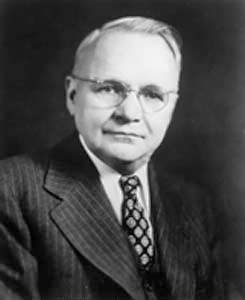
\includegraphics[width=2.71in]{../figures/Harry_Nyquist.jpg}
			\caption{Picture of Harry Nyquist from the American Institute of Physics. \bl{Fair use, via Wikimedia Commons}}
			\label{fig:fragility_curve}
		\end{figure}


\end{review}

\subsection{Experimental Signal Processing}

\todo{to be updated based on Open Vibrations}
\begin{figure}[H]
    \centering
    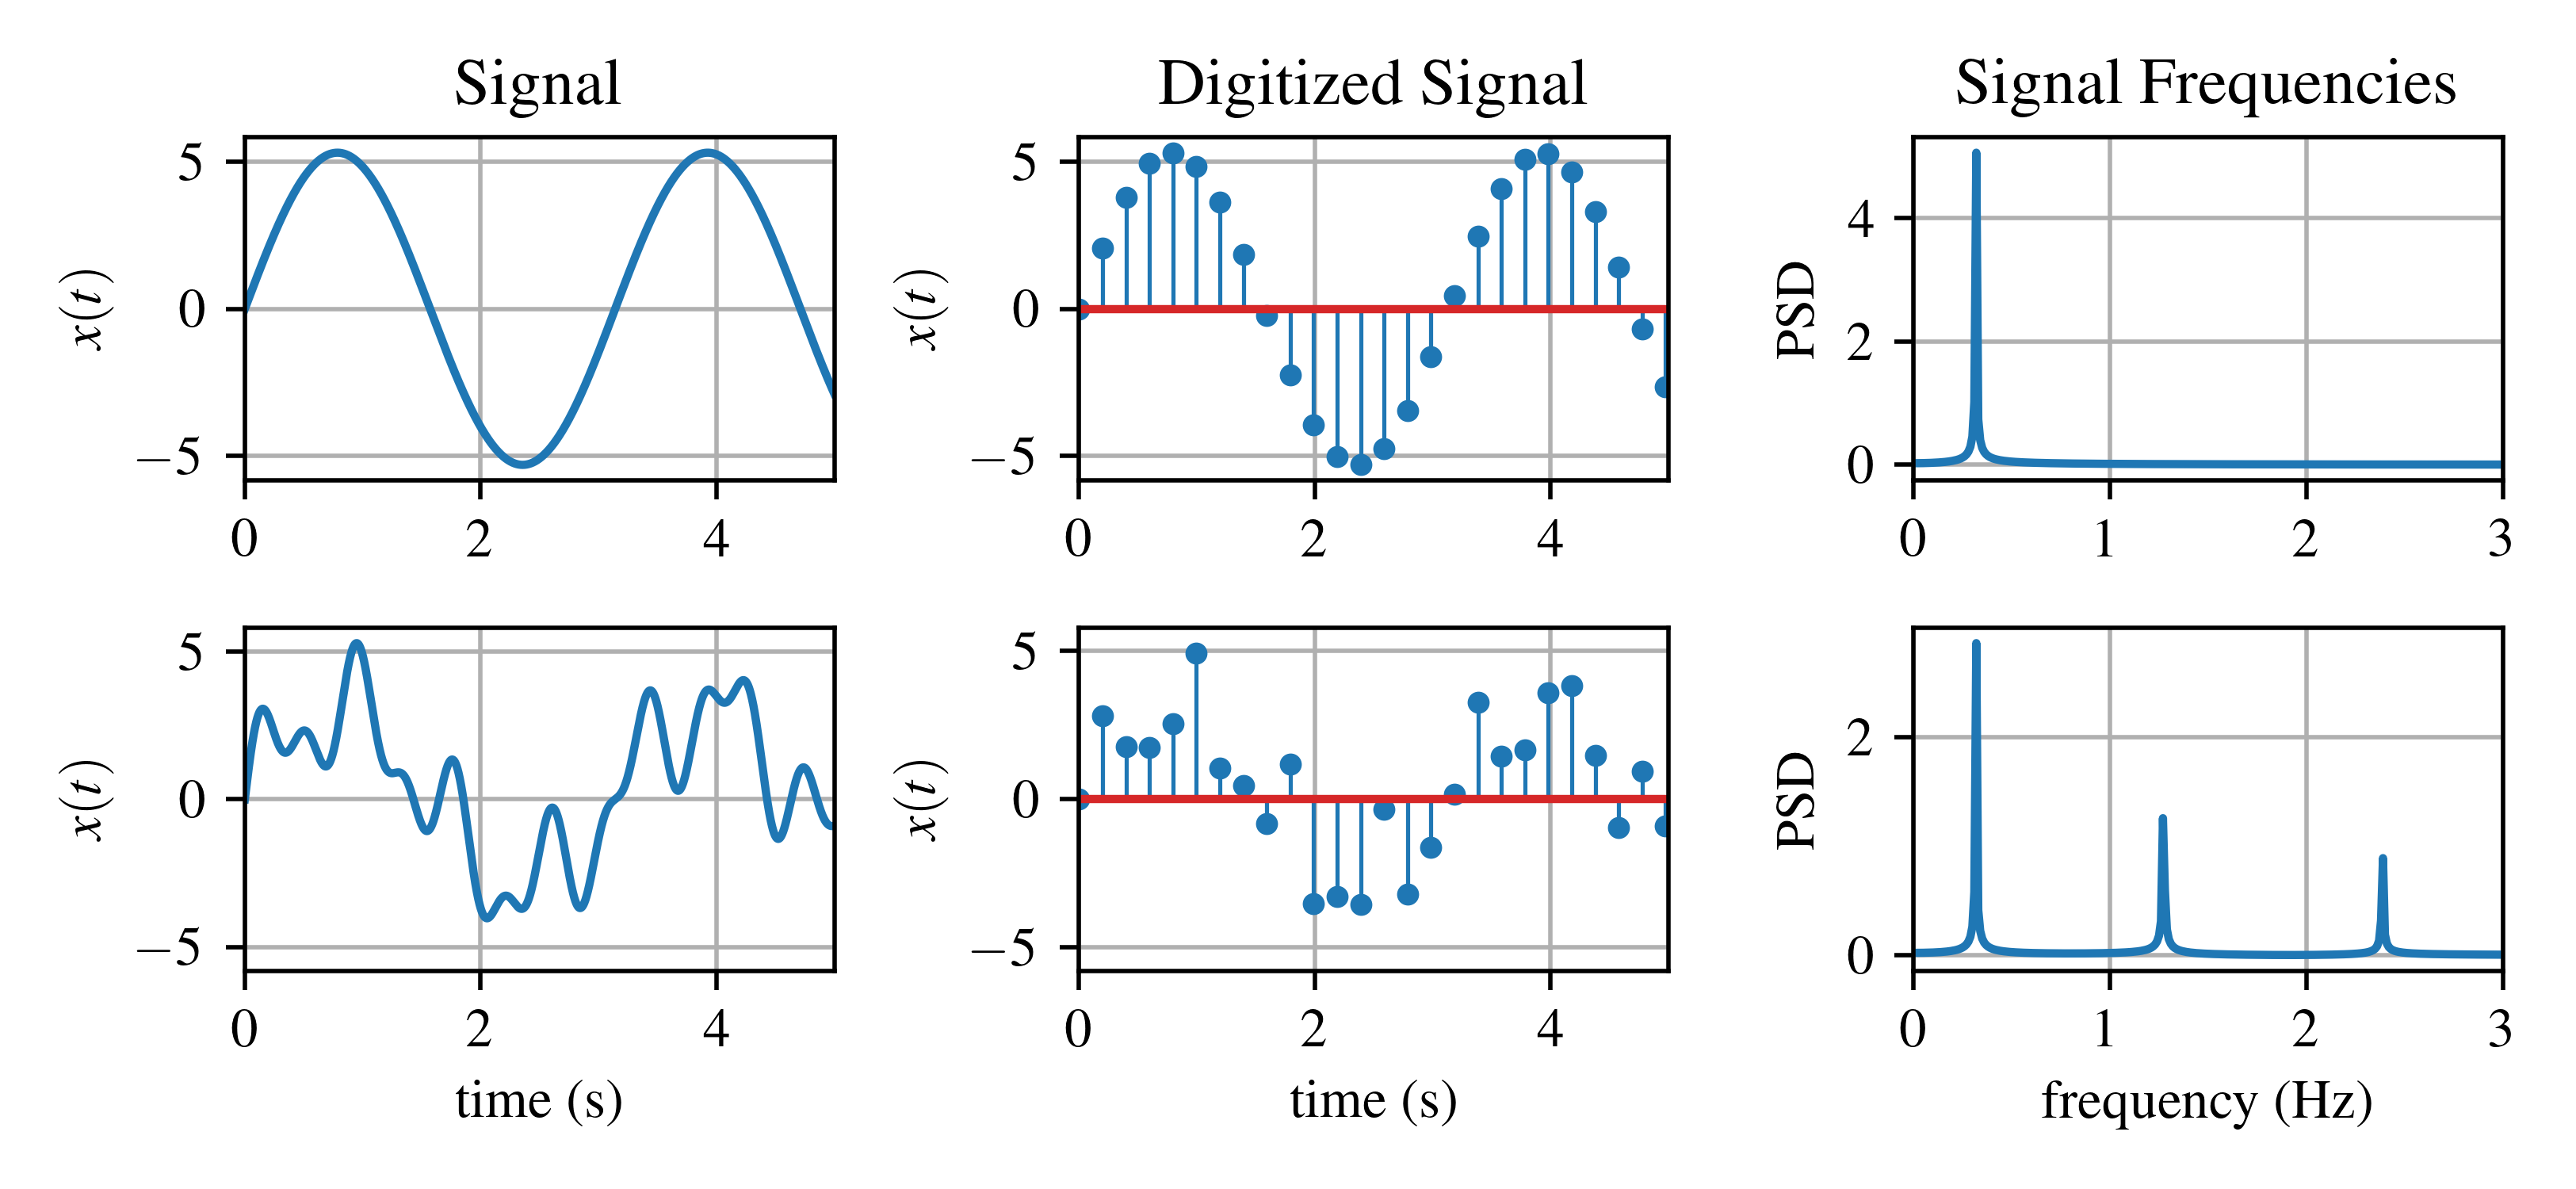
\includegraphics[width=6.5in]{../figures/signal_digitization.png}
    \caption{Digitization of two continuous time-series signals sampled at 5 S/s.}
    \label{fig:signal_digitization}
\end{figure}


The Nyquist-Shannon sampling theorem is a theorem in the field of signal processing that defines the sample rate that permits a discrete sequence of samples (i.e. discrete-time) to sample a continuous-time signal of a finite bandwidth. 

\begin{figure}[H]
    \centering
    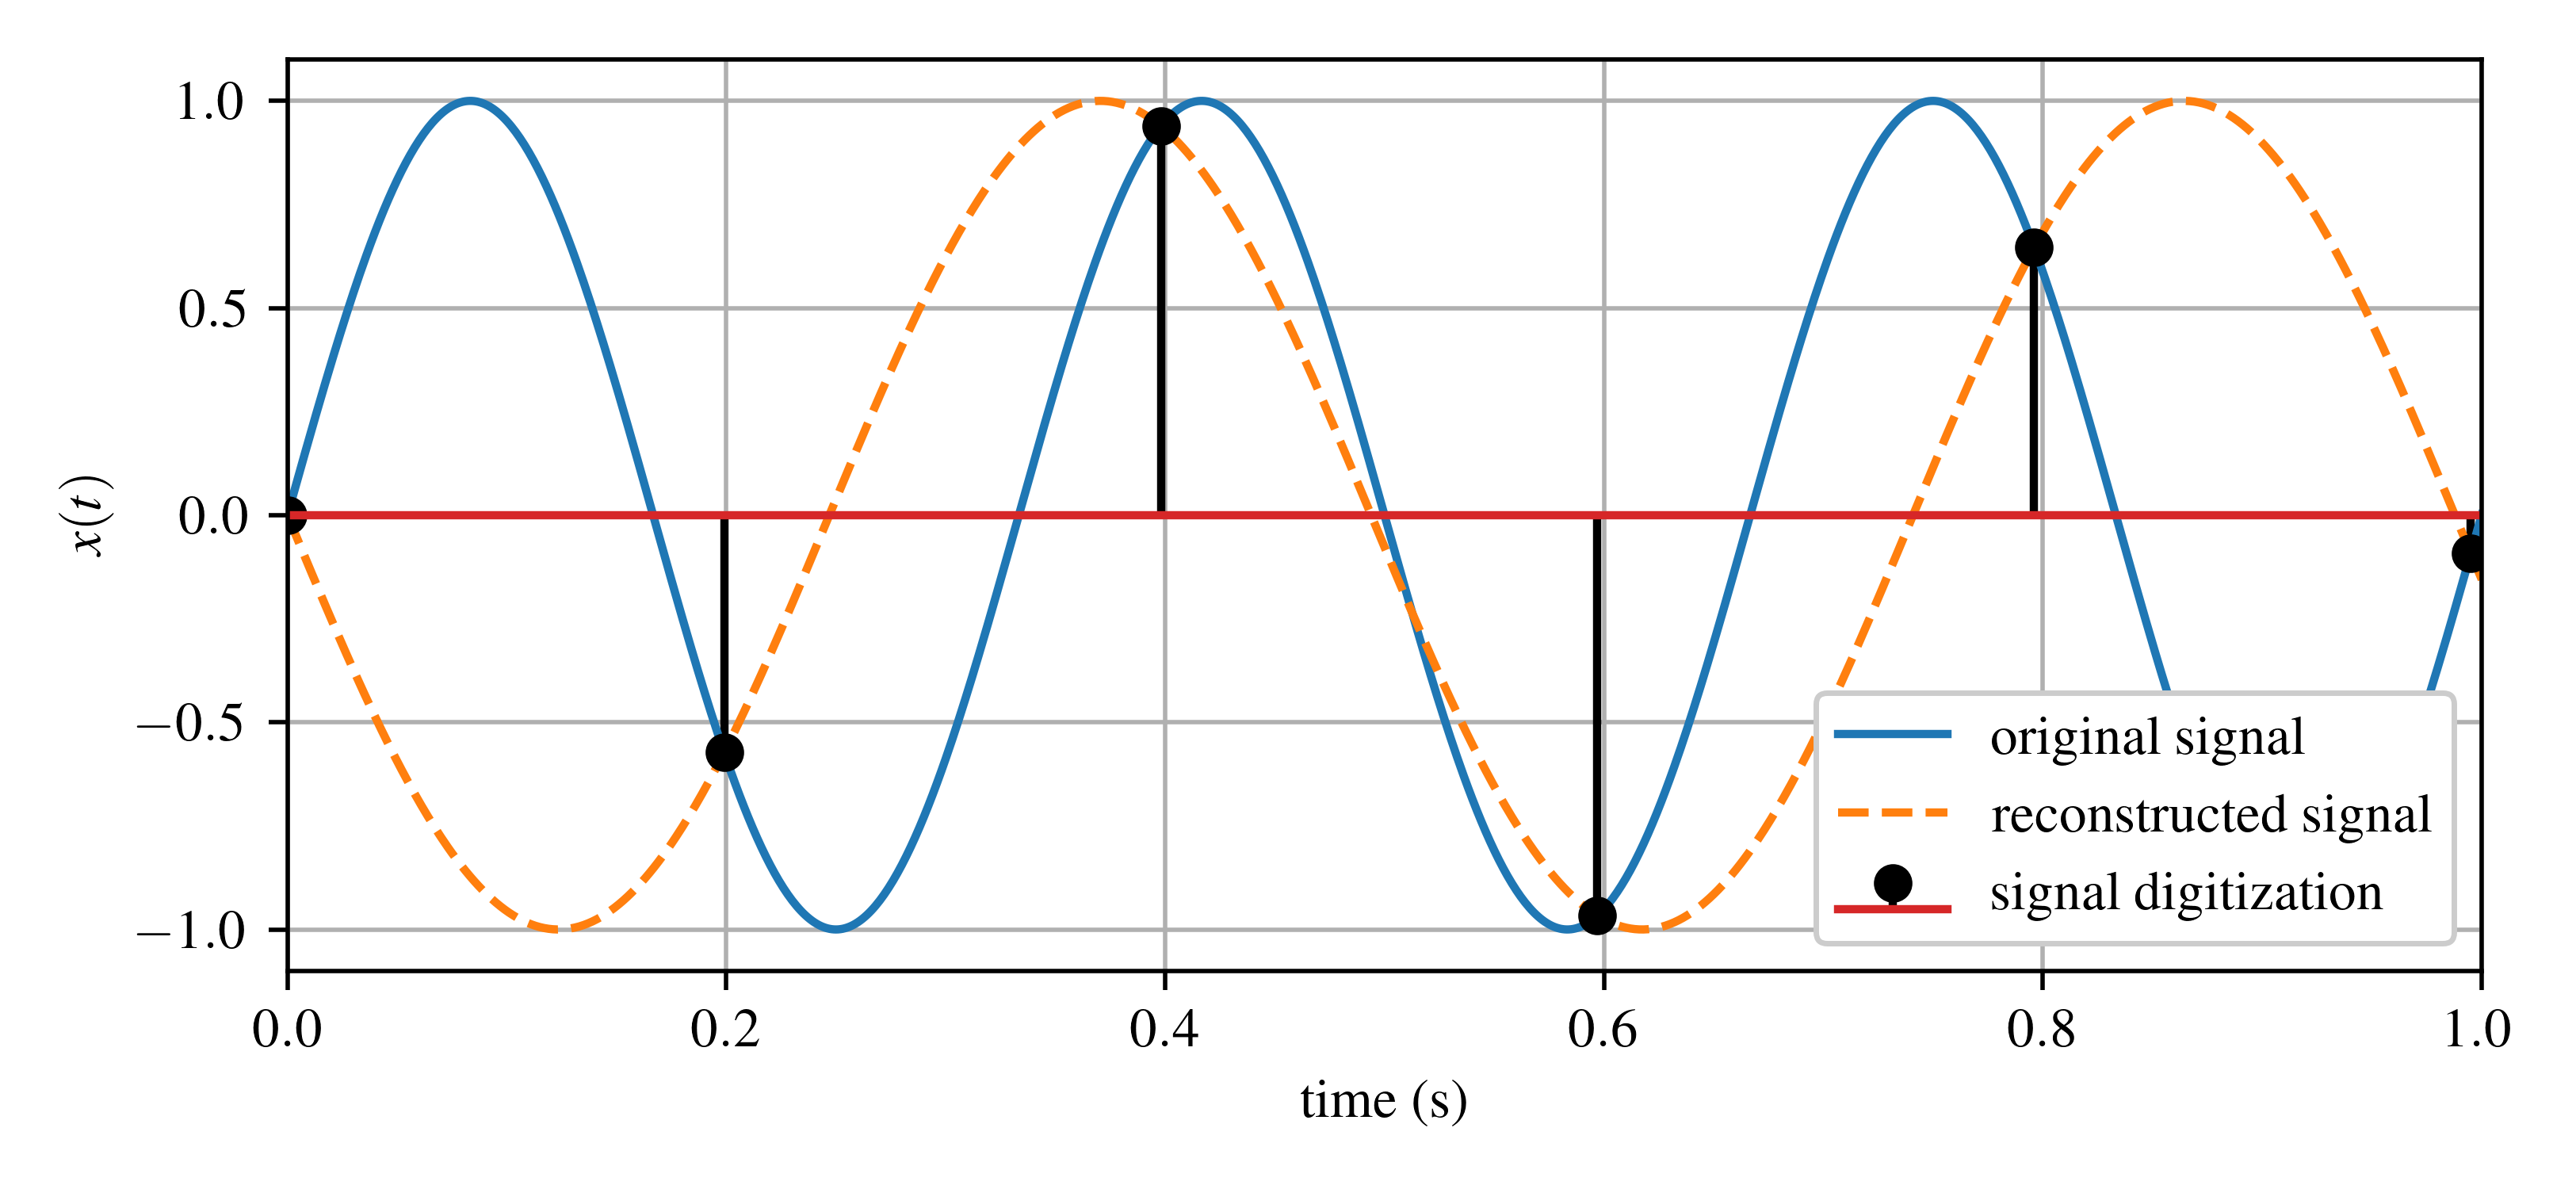
\includegraphics[width=6.5in]{../figures/aliasing.png}
    \caption{Aliasing of a 3 Hz signal that is sampled at 5 S/s.}
    \label{fig:aliasing}
\end{figure}

In signal processing, aliasing is an effect that causes different signals to become indistinguishable from each other.  In this way, the signals become an aliases of one another when sampled. Aliasing also accounts for the development of distortion or artifact in a reconstructed signal when compared to the original continuous signal.


\subsection{System Identification for 1\textsuperscript{st}-order systems}



\begin{figure}[H]
    \centering
    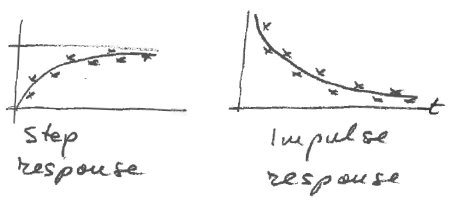
\includegraphics[width=3.5in]{../figures/system_ID_experimental}
\end{figure}

Given a 1\textsuperscript{st}-order system subjected to either a step or impulse input, there is a need to find the time constant ($T$) for the first-order transfer function
\begin{equation}
G(s) = \frac{1}{Ts+1}
\end{equation}

\subsubsection{Option 1 Optimization} 

Here, the task is to fit a curve to the experimental data. To do this, minimize the error in the function
\begin{equation}
x(t;T) = 1-e^{-t/T}
\end{equation}
for a series of experiments
\begin{align}
x_\text{exp} &= x_1, \; x_2, \; x_3, \cdots \\
t_\text{exp} &= t_1, \; t_2, \; t_3, \cdots  \nonumber
\end{align}
using any number of available curve fitting software to find $T$. 

\todo{add example with curve fitting in Matlab}

\subsubsection{Option 2 Graphical Methods}

In this method graphical methods can be used to provide quick estimates of the system parameter. 
\begin{itemize}
\item \textbf{Tangent at Origin} This method shows us that $T = t_\text{A}$, as shown in the figure
\begin{figure}[H]
    \centering
    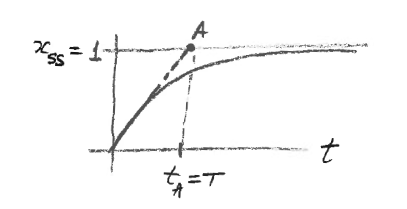
\includegraphics[width=3in]{../figures/tangent_at_origin_method}
\end{figure}
\begin{equation}
x(t) = 1-e^{-t/T}
\end{equation}
and 
\begin{equation}
\dot{x} = \frac{dx}{dt} = \bigg(-\frac{1}{T}\bigg)\bigg(-e^{-t/T}\bigg) = \frac{1}{T}e^{-t/T}
\end{equation}
therefore
\begin{equation}
\dot{x}_0 = \frac{dx}{dt}\big|_{t=0} = \frac{1}{T}
\end{equation}
therefore, the tangent at the origin is 
\begin{equation}
y(t) = \dot{x}_0 t = \frac{1}{T} t
\end{equation}
where $y(t)$ intersects $x_{ss}=1$ at $\frac{1}{T} t_\text{A}=1$; therefore 
\begin{equation}
T = t_\text{A}
\end{equation}
\item \textbf{Half Time} Thought measuring the half time of a 1\textsuperscript{st}-order systems subjected to either a step or impulse input, the time constant can be obtained. 
\begin{figure}[H]
    \centering
    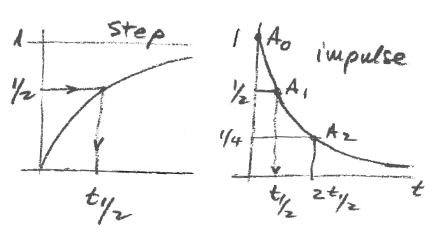
\includegraphics[width=3.5in]{../figures/half_time_method}
\end{figure}
\begin{itemize}
\item For a step function
\begin{equation}
x(t) = 1-e^{-t/T}
\end{equation}
solving for $t$ = $t_{1/2}$ leads to
\begin{align}
x(t_{1/2}) &= 1/2 \\
1/2 &= 1-e^{-t_{1/2}/T} \nonumber \\
&= e^{-t_{1/2}/T} \nonumber
\end{align}
solving for $T$ results in
\begin{align}
\frac{-t_{1/2}}{T} &= \ln(1/2) \\
T &= \frac{-t_{1/2}}{\ln(1/2)} \nonumber \\
 &= \frac{t_{1/2}}{0.693} \nonumber \\
 &\approxeq 1.4 t_{1/2} \nonumber 
\end{align} 
\item For a impulse function
\begin{equation}
x(t) = \frac{1}{T}e^{-t/T}
\end{equation}
where
\begin{align}
x(t_{1/2}) &= 1/2 \\
1/2 &= \frac{1}{T}e^{-t_{1/2}/T} \nonumber
\end{align}
therefore
\begin{align}
T &= \frac{-t_{1/2}}{\ln(1/2)} \nonumber \\
T &\approxeq 1.4 t_{1/2} \nonumber 
\end{align} \todo{This equation is correct, but I don't have a proof for it. }
Note that you may use the consecutive points $A_1$, $A_2$ if $A_0$ is not easy to determine, important is that signal halves between $A_1$ and $A_2$. 



\begin{mdframed}[middlelinewidth=0.5mm]
	\begin{center}
		\gr{Proof}
	\end{center}
For the expression
\begin{align}
x(t_{1/2}) &= 1/2 \\
1/2 &= 1-e^{-t_{1/2}/T} \nonumber \\
&= e^{-t_{1/2}/T} \nonumber
\end{align}
we can show \rd{the rest of this is only true for T=1, need a more robust proof.}
\begin{equation}
T=-\frac{t_{1/2}}{W_0 \big(-\frac{t_{1/2}}{2}\big)}
\end{equation}
where $W_0$ is the upper branch of the Lambert Function and $W_0\big(-\frac{t_{1/2}}{2}\big) \neq 0$, $t_{1/2} \neq 0 $ and $n \in \mathbb{Z} $
\begin{figure}[H]
    \centering
    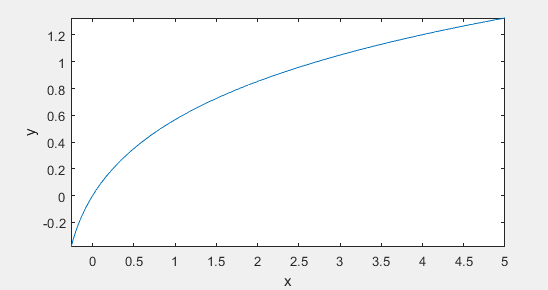
\includegraphics[width=3.5in]{../figures/Lambert_function}
	\caption{The upper branch of the Lambert Function graphed for $y = W_0(x)$ for real components. }
\end{figure}

\end{mdframed}




\end{itemize}
\end{itemize}

\subsubsection{Option 3 Performance Indicators}
 
Two methods can be used to estimate the time period:
\begin{itemize}
\item \textbf{Delay time} ($t_d$) can be used to estimate the time period, as 
\begin{equation}
t_d = -T \ln(0.5)
\end{equation}
and therefore
\begin{equation}
T = - \frac{t_d}{\ln(0.5)}
\end{equation}
\item \textbf{Settling time} $t_s$ can be uses to estimate the time period, here consider the 2\% settling time value 
\begin{equation}
t_s^{2\%} = -T \ln(0.02)
\end{equation}
and therefore
\begin{equation}
T = - \frac{t_s^{2\%}}{\ln(0.5)}
\end{equation}
\end{itemize}

\subsection{System Identification for 2\textsuperscript{nd}-order systems}

\begin{figure}[H]
    \centering
    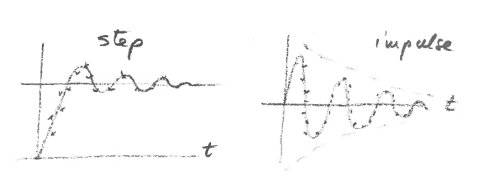
\includegraphics[width=4.5in]{../figures/2nd_order_system_ID_experimental}
\end{figure}

Given a 2\textsuperscript{nd}-order system subjected to either a step or impulse input, there is a need to find the natural frequency ($\omega_n$) and damping ratio ($\zeta$) for the 2\textsuperscript{nd}-order transfer function
\begin{equation}
G(s) = \frac{\omega_n^2}{s^2 + 2 \zeta \omega_n s + \omega_n^2}
\end{equation}

\subsubsection{Optimization}

Here, the task is to fit a curve to the experimental data. To do this, minimize the error in the time series response of the system for a series of experiments
\begin{align}
x_\text{exp} &= x_1, \; x_2, \; x_3, \cdots \\
t_\text{exp} &= t_1, \; t_2, \; t_3, \cdots  \nonumber
\end{align}
using any number of available curve fitting software to find the natural frequency ($\omega_n$) and damping ratio ($\zeta$). 

%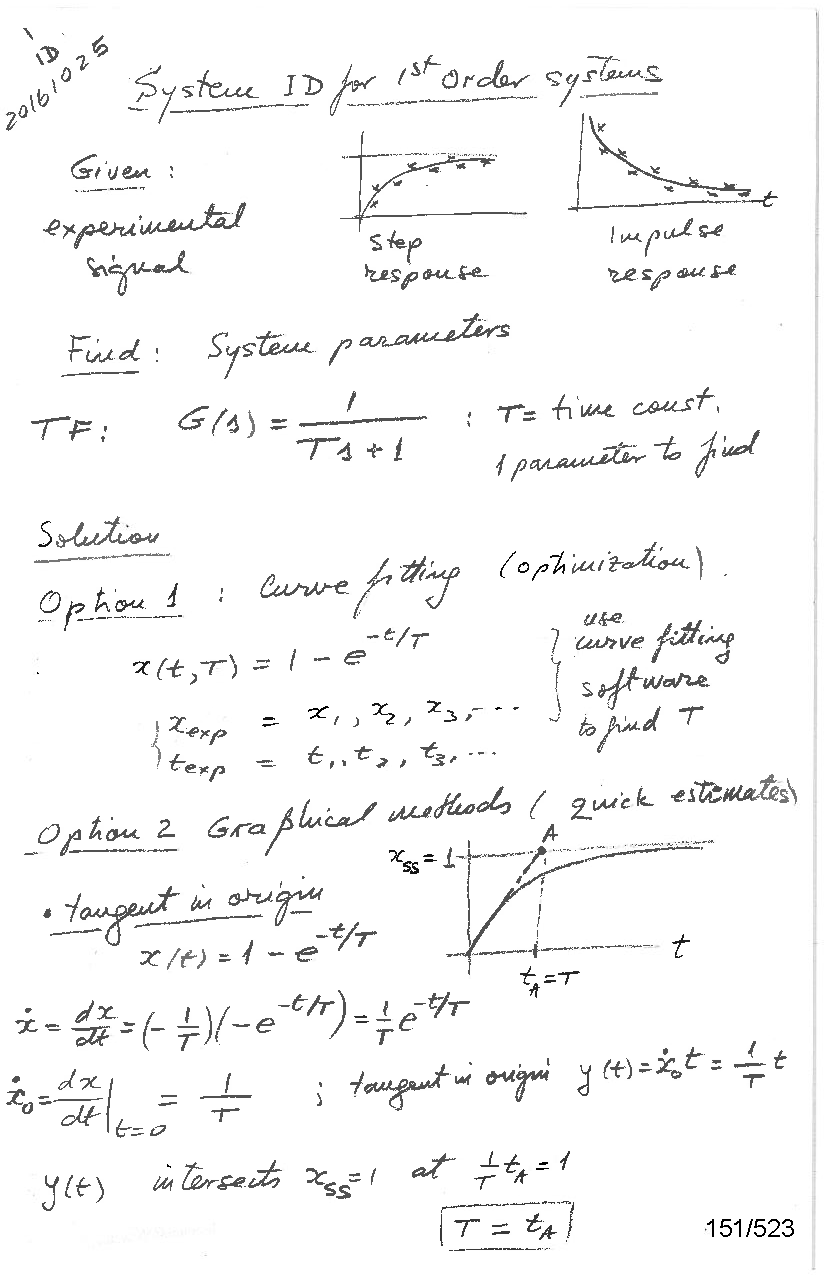
\includepdf[pages=-,pagecommand={},width=0.9\textwidth]{PDF_notes/System_Identification.pdf}
\todo{add Matlab example, maybe with beam.}

	
\subsubsection{Frequency Estimation} Can be performed by finding the frequency at which the damped system crosses a given point, termed at $f_d$. This is either
\begin{itemize}
\item \textbf{Peak Detection} 
			\begin{figure}[H]
				\centering
				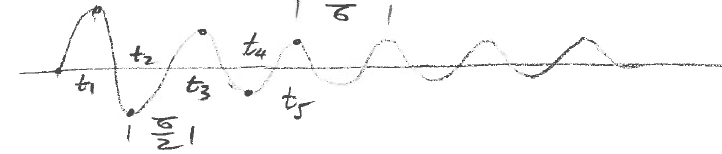
\includegraphics[width=5in]{../figures/peak_detection.png}
			\end{figure}	
Is done by taking the average of the half period
\begin{equation}
f_d = \frac{\tau}{2} = \text{avg}\big[ (t_2-t_1), (t_2-t_1), \cdots \big]
\end{equation}
\item \textbf{Zero Crossing} 
			\begin{figure}[H]
				\centering
				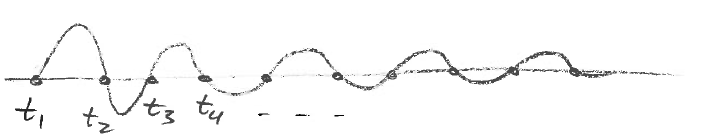
\includegraphics[width=5in]{../figures/zero_crossing.png}
			\end{figure}
\end{itemize}	
Is done by taking the average of the half period
\begin{equation}
f_d = \frac{\tau}{2} = \text{avg}\big[ (t_2-t_1), (t_2-t_1), \cdots \big]
\end{equation}
In either case, 
\begin{equation}
\omega_d = 2 \pi f_d
\end{equation}
where 
\begin{equation}
f_n = \frac{f_d}{\sqrt{1-\zeta^2}}
\end{equation}
and
\begin{equation}
\omega_n = 2 \pi f_n
\end{equation}


\subsubsection{Step Response Analysis ($\zeta << 1$)}
			\begin{figure}[H]
				\centering
				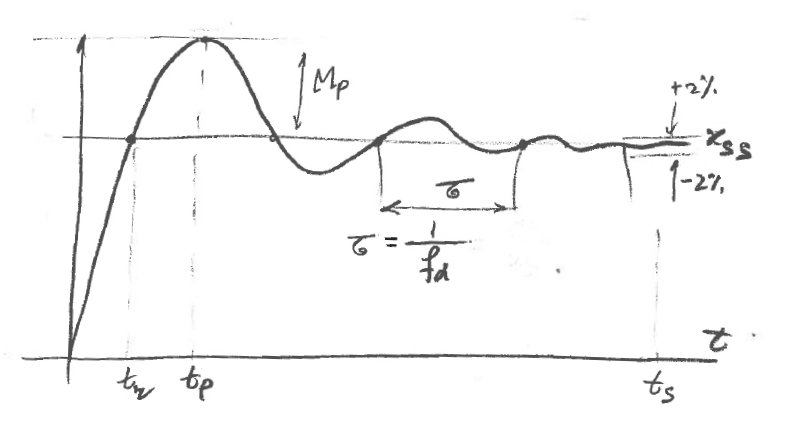
\includegraphics[width=5in]{../figures/system_identification_step_response.png}
			\end{figure}

Recall that the rise time is
\begin{equation}
t_r = \frac{\pi - \phi}{\omega_n \sqrt{1-\zeta^2}} = \frac{\pi - \phi}{\omega_d}
\end{equation}
with
\begin{equation}
\omega_d = \omega_n \sqrt{1-\zeta^2}
\end{equation}
and
\begin{equation}
\phi = \tan^{-1} \frac{\sqrt{1-\zeta^2}}{\zeta} = \sin^{-1} \sqrt{1-\zeta^2}
\end{equation}
while peak time is
\begin{equation}
t_p = \frac{\pi}{\omega_n \sqrt{1-\zeta^2}} = \frac{\pi}{\omega_d}
\end{equation}
The max percentage overshoot is
\begin{equation}
M_p  = e^{- \frac{\zeta}{\sqrt{1-\zeta^2}} \pi }= \frac{x_p - x_{ss}}{x_{ss}} 100\%
\end{equation}
and lastly, settling time is
\begin{equation}
t_s \approxeq \frac{4}{\zeta \omega_n}
\end{equation}
From this, there are only two unknowns, $\omega_n$ and $\zeta$. There is more information than minimally required to obtain these from $t_r$, $t_p$, $M_p$,and $t_s$.

\begin{itemize}
\item Obtain $\omega_n$ and $\zeta$ from $t_r$ and $t_p$.  
\begin{equation}
t_p = \frac{\pi}{\omega_d} \rightarrow \omega_d = \frac{\pi}{t_p}
\end{equation}
and
\begin{align}
t_r  = \frac{\pi - \phi}{\omega_d} \rightarrow \phi &= \pi - t_r \omega_d  \\
 &= \pi -\frac{t_r}{t_p} \pi \nonumber \\
 &= \pi(1-\frac{t_r}{t_p}) \nonumber 
\end{align}
recall that 
\begin{align}
\phi &= \sin^{-1} \sqrt{1-\zeta^2} \\
1-\zeta^2 &= \sin^2 \phi \nonumber \\
\zeta &= \sqrt{1-\big[\sin (\phi)\big]^2}
\end{align}
and
\begin{equation}
\omega_n = \frac{\omega_d}{\sqrt{1-\zeta^2}}
\end{equation}
\item  Obtain $\zeta$ from $M_p$.  
\begin{align}
M_p  &= e^{- \frac{\zeta}{\sqrt{1-\zeta^2}} \pi } \\
- \frac{\zeta}{\sqrt{1-\zeta^2}} \pi  &= \ln(M_p) \nonumber \\
\zeta^2 \pi^2 &= (1-\zeta^2)\big(\ln(M_p)\big)^2  \nonumber \\
\zeta^2 \pi^2 &= \big(\ln(M_p)\big)^2  - \zeta^2 \big(\ln(M_p)\big)^2  \nonumber \\
\zeta^2 \bigg[\pi^2 + \big(\ln(M_p)\big)^2 \bigg] &= \big(\ln(M_p)\big)^2   \nonumber \\
\zeta^2 &= \frac{(\ln(M_p))^2}{\pi^2 + \big(\ln(M_p)\big)^2 }    \nonumber \\
\zeta &= \frac{|\ln(M_p)|}{\sqrt{\pi^2 + \big(\ln(M_p)\big)^2 }}    \nonumber
\end{align}
\item Obtain $\omega_n$ and $\zeta$ from $t_p$ and $t_s$.  
\begin{equation}
t_p = \frac{\pi}{\omega_d} \rightarrow \omega_d = \frac{\pi}{t_p}
\end{equation}
next
\begin{align}
\omega_n &= \frac{\omega_d}{\sqrt{1-\zeta^2}} \\
&= \frac{\frac{\pi}{t_p}}{ \sqrt{1-\zeta^2}}  \nonumber \\
&= \frac{\pi}{t_p \sqrt{1-\zeta^2}} \nonumber 
\end{align}
looking at the settling time
\begin{align}
t_s &= \frac{4}{\zeta \omega_n}  \\
&= \frac{4 t_p \sqrt{1-\zeta^2}}{\zeta \pi} \nonumber \\
t_s \zeta \pi &= 4 t_p \sqrt{1-\zeta^2} \nonumber \\
t_s^2 \zeta^2 \pi^2 &= 16 t_p^2(1- \zeta^2) \nonumber \\
(16 t_p^2-\pi^2 t_s^2) \zeta^2 &= 16 t_p \nonumber \\
\zeta^2 &= \frac{16 t_p}{16 t_p^2-\pi^2 t_s^2} \nonumber \\
 &= \frac{1}{1-\big(\frac{\pi}{4}\frac{t_s}{t_p}\big)^2} \nonumber \\
\zeta &= \frac{1}{\sqrt{1-\big(\frac{\pi}{4}\frac{t_s}{t_p}\big)^2}} \nonumber 
\end{align}
\item Obtain $\omega_n$ and $\zeta$ from $M_p$ and $t_r$.  
\begin{equation}
\zeta = \frac{|\ln M_p|}{\sqrt{\pi^2 + (\ln M_p)^2}}
\end{equation}
Recall that 
\begin{equation}
t_r = \frac{\pi - \phi}{\omega_n \sqrt{1-\zeta^2}} = \frac{\pi - \phi}{\omega_d}
\end{equation}
Therefore
\begin{equation}
\omega_n = \frac{\pi - \phi}{t_r \sqrt{1-\zeta^2}}
\end{equation}
where 
\begin{equation}
\phi = \sin^{-1} \sqrt{1-\zeta^2}
\end{equation}
\end{itemize}


% \subsection{Measuring Performance Indicators in SIMULINK}

System identification can be done through measuring performance indicators using Simulink.

\begin{example}

\textbf{SIMULINK Tutorial on Measuring Performance Indicators}

System identification can be done through measuring performance indicators using Simulink. Consider a 2\textsuperscript{nd}-order system with $k=700$ N/m, $c=15$ kg/s, and $m=7$ kg. To implement this in Simulink, one could use MATLAB to generate the transfer function:

\lstset{linewidth=5.8in}
\begin{minipage}{1\textwidth}
  \begin{center}
    \lstset{%
caption={MATLAB code for Method II.},
      basicstyle=\ttfamily\footnotesize\bfseries,
      frame=tb,
    }
\begin{lstlisting}
%% calculate system values
c = 15;     % N/(m/sec)
k = 700;    % N/m,
m = 7;      % kg
w_n = sqrt(k/m)     % natural frequency in rad/sec
z = c/(2*sqrt(k*m)) % damping ratio
w_d = w_n*sqrt(1-z^2);   % damped natural frequency in rad/sec

%% calculate transfer function G(s)
B = [w_n^2];
A = [1 2*z*w_n w_n^2];
G = tf(B,A) % build the transfer function
\end{lstlisting}
  \end{center}
\end{minipage}

and than deploy the transfer function to SIMULINK as shown below
\begin{figure}[H]
	\centering
	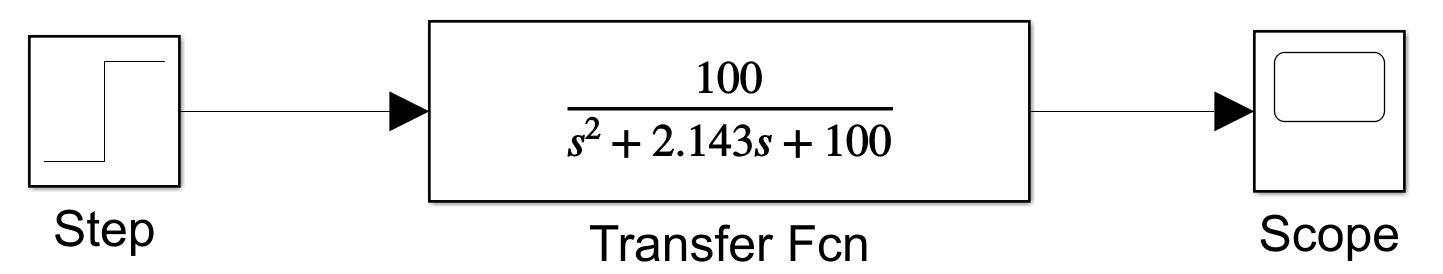
\includegraphics[width=4.5in]{../figures/Simulink_step_model_transfer_2nd_oder_2}
\end{figure}

Using the scope and waveform cursors, several performance indicators can be read
\begin{figure}[H]
	\centering
	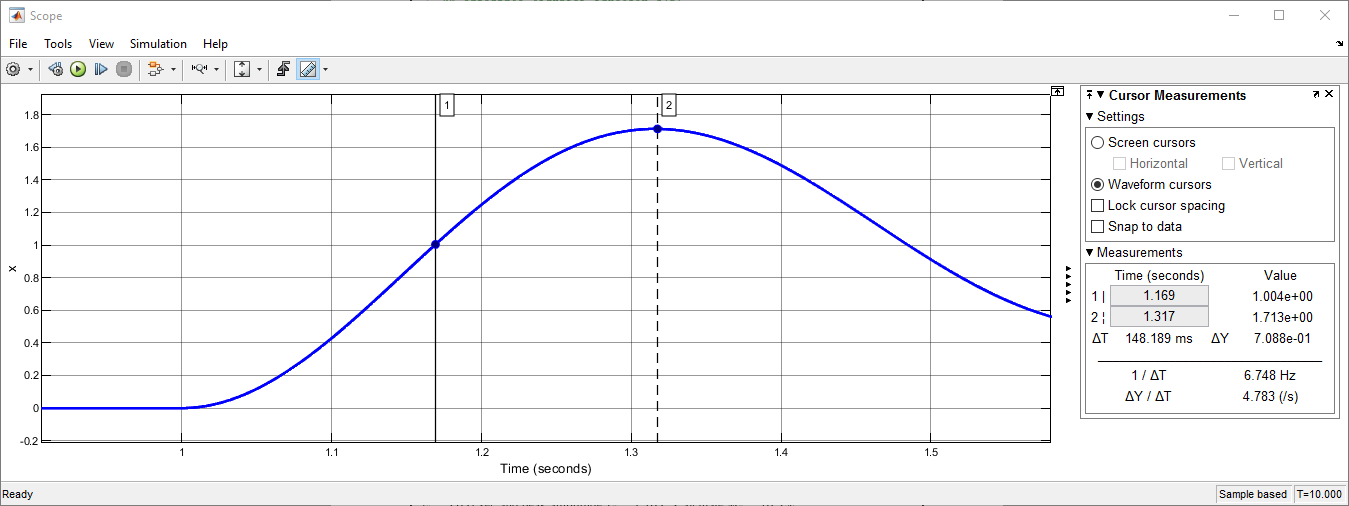
\includegraphics[width=6.0in]{../figures/Simulink_step_model_transfer_cursor_measurements_2nd_oder_2}
\end{figure}
these include
\begin{itemize}
\item $t_r = 0.169$ sec
\item $t_p = 0.317$ sec
\item $x_p = 1.173$ m
\item $M_p = 71.3\%$
\end{itemize}

From these, measurements the damping ratio of the system can be obtained using one of two methods, 
\begin{itemize}
\item \textbf{Method 1} Estimate damping ratio using $t_r$ ,$t_p$. Knowing that 
\begin{align}
\phi &= \pi(1-t_r/t_p) \\
&= 1.46674 \nonumber \\
\end{align}
and 
\begin{align}
\zeta &= \sqrt{1-\big[\sin (\phi)\big]^2} \\
&= 0.1039 \nonumber \\
\end{align}
\item \textbf{Method 2} Estimate damping ratio using $M_p$. Knowing that 
\begin{align}
\zeta &= \frac{|\ln M_p|}{\sqrt{\pi^2 + (\ln M_p)^2}} \\
&= \frac{|\ln (0.72)|}{\sqrt{\pi^2 + (\ln M0.72)^2}} \nonumber \\
&=  0.1071 \nonumber \\
\end{align}
These values give an error of 3.4\% and 0\% when compared to the correct value of $\zeta = 0.1071$, respectively. This is considered very good, but these are ideal systems with no noise and therefore excellent predictions are to be expected. 
\end{itemize}

The SIMULINK model can also be used to estimate the natural frequency of the system using the zero crossing method by placing the coursers as close as possible to the ``zero'' value, 1 cycle apart. Here, ``zero'' is one due to the system being subjected to a step response.
\begin{figure}[H]
	\centering
	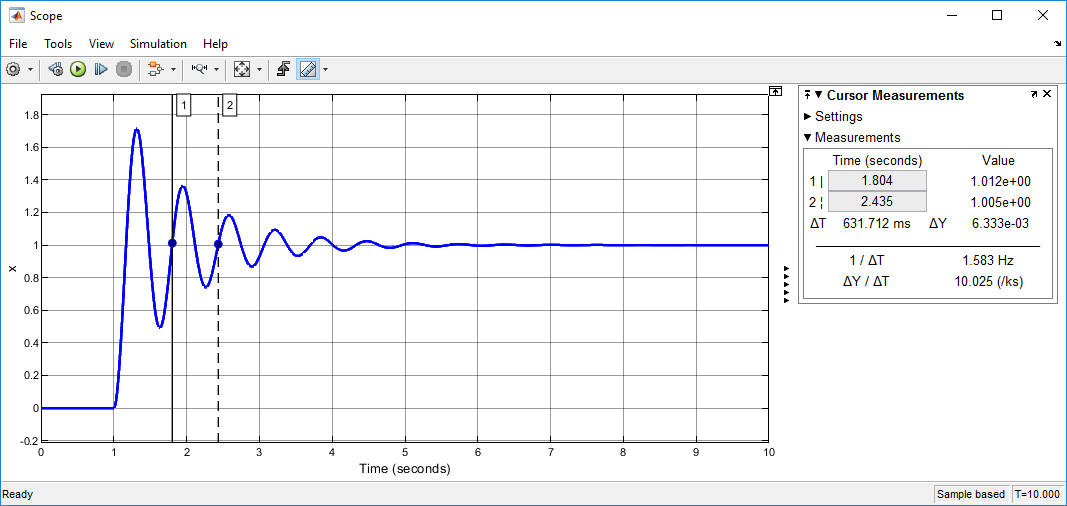
\includegraphics[width=6.0in]{../figures/Simulink_step_model_transfer_cursor_measurements_2nd_oder_3}
\end{figure}
The $\Delta T$ of the cursors is 0.631712 sec, or 1.583 Hz. This is 0.53\$ off from the true value of 1.5915 Hz. 
\end{example}







\subsubsection{Logarithmic decrement}



Logarithmic decrement ($\zeta << 1$) For a vibrating system, the  mass ($m$) and stiffness ($k$) can be measured using scales and static deflection tests. However, the damping coefficient ($c$) is a more difficult quantity to determine. From $k$ and $m$ we can compute the natural frequency ($\omega_\text{n}$) and the critical damping coefficient ($c_\text{cr}$). Therefore, knowing that the critical damping ratio ($\zeta$) is defined as:
			\begin{equation}
				\zeta = \frac{c}{c_{\text{cr}}} = \frac{c}{2\sqrt{km}} = \frac{c}{2m\omega_\text{n}}
			\end{equation}				
			if we calculate $\zeta$, we can obtain $c$ for the system of interest. This is made possible because $c_\text{cr}$ can be calculated from $k$ and $m$. Observing the temporal response for the underdamped system, 

	        \begin{minipage}{\linewidth}
	            \centering
	            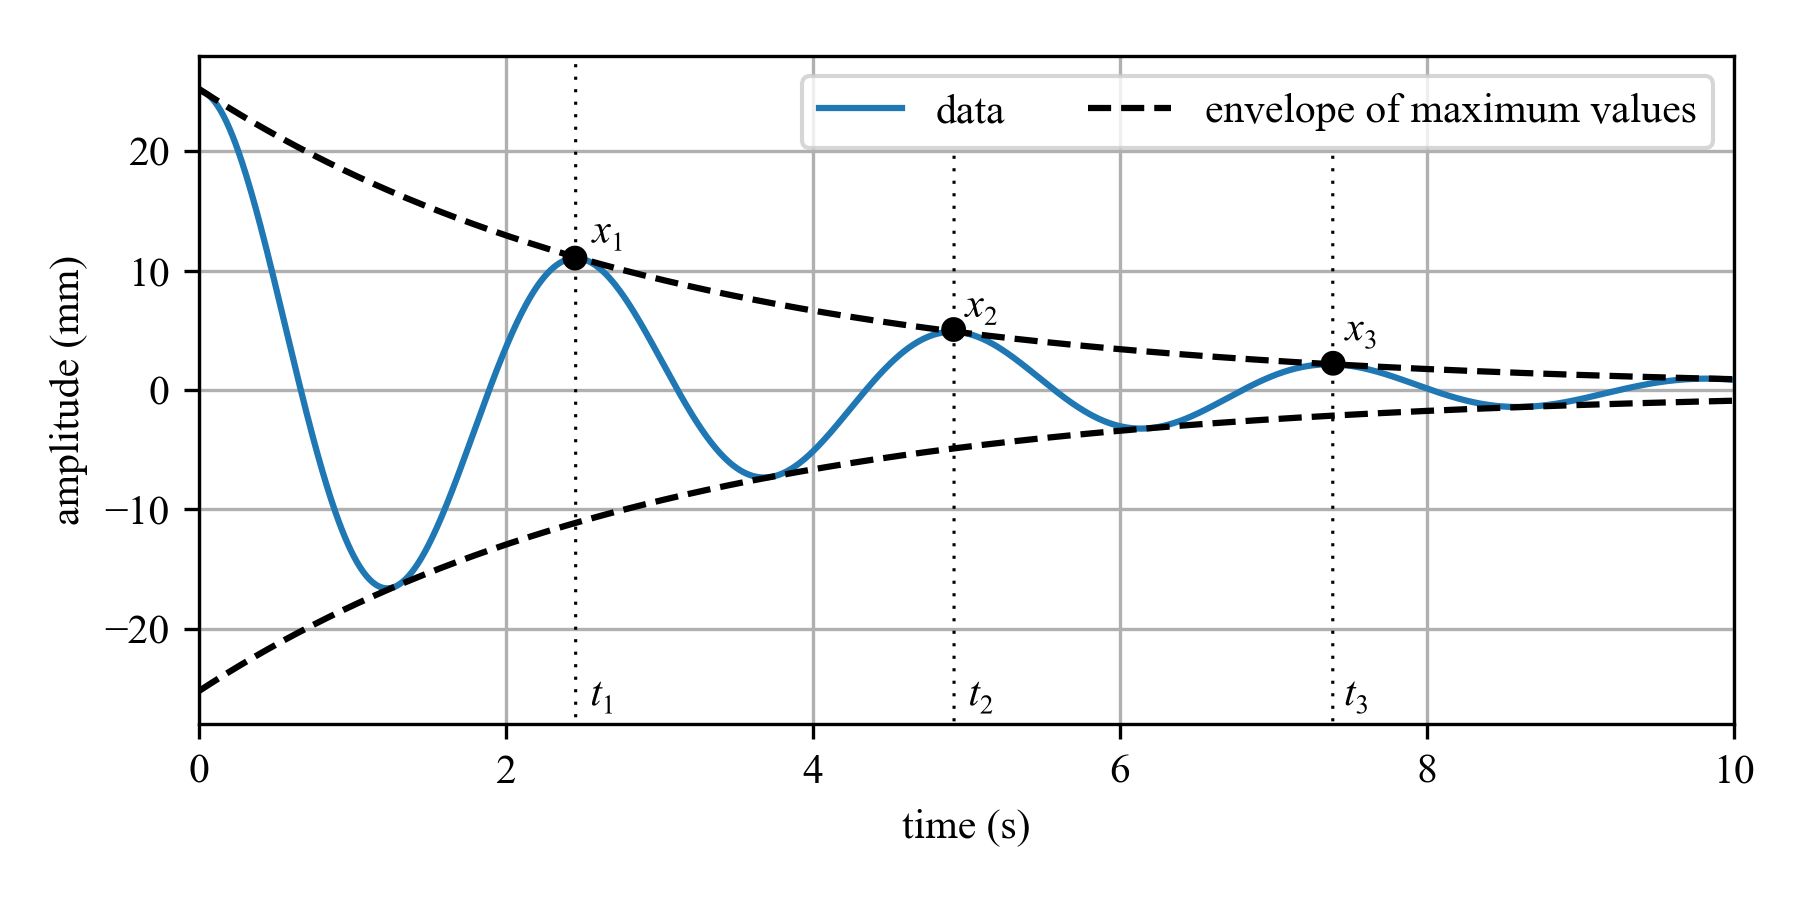
\includegraphics[width=\linewidth]{../figures/Logarithmic_decrement.png}
	            \captionof{figure}{Measuring the peak displacements points in an experimental system with decay caused by damping.}
	        \end{minipage}
			
			\noindent we mark three points of maximum amplitude, $x_1$, $x_2$, and $x_3$ that happen at $t_1$, $t_2$, and $t_3$, respectively. Considering displacement values for the first two points $x_1$ and $x_2$, separated by a complete period ($T$).  Knowing that one cycle is $2 \pi$, the time period for this complete cycle is given by:
			\begin{equation}
				t_2-t_1 = \frac{2\pi}{\omega_\text{d}} = \frac{2\pi}{\omega_\text{n}\sqrt{1-\zeta^2}}
			\end{equation}				
			where $\omega_\text{d}$ is the damped natural frequency. This is the time period ($T$) of damped oscillations. If we derive an equation for the values of the peaks, also called the envelope of maximum values, we get: 
			\begin{equation}
				x_{\text{peaks}} = Ae^{-\zeta\omega_\text{n}t} 
			\end{equation} 		
			Knowing that the system is underdamped, $A$ can be solved for using the initial conditions $x_0$ and $v_0$, therefore: 
			\begin{equation}
				A = \frac{\sqrt{(v_0+\zeta\omega_\text{n}x_0)^2 + (x_0\omega_\text{d})^2}}{\omega_\text{d}}
			\end{equation} 	
			In terms of $t_1$ and $t_2$, we can express the displacement at these times as:
			\begin{equation}
				x_{\text{1}} = A e^{-\zeta \omega_\text{n} t_1}
			\end{equation}				
			and 
			\begin{equation}
				x_{\text{2}} = A e^{-\zeta \omega_\text{n} t_2}
			\end{equation}		
			therefore:
			\begin{equation}
				\frac{x_{\text{1}}}{x_{\text{2}}} = \frac{e^{-\zeta \omega_\text{n} t_1}}{e^{-\zeta \omega_\text{n} t_2}} = e^{\zeta \omega_\text{n}(t_2-t_1)}
			\end{equation}		
			However, from before we know that $t_2-t_1 = \frac{2\pi}{\omega_\text{d}} = \frac{2\pi}{\omega_\text{n}\sqrt{1-\zeta^2}}$. Therefore, we can express this last equation as:
			\begin{equation}
				\frac{x_{\text{1}}}{x_{\text{2}}} =e^{\Big(\frac{2 \pi \zeta}{\sqrt{1-\zeta^2}}\Big)}
			\end{equation}			
			Next, we take the natural log of both sides to get the logarithmic decrement, denoted by $\delta$:
			\begin{equation}
				\delta = \text{ln}\bigg(\frac{x_{\text{1}}}{x_{\text{2}}}\bigg) = \text{ln}\bigg(\frac{x(t_{\text{1}})}{x(t_{\text{1}}+T)}\bigg) = \frac{2 \pi \zeta}{\sqrt{1-\zeta^2}}
			\end{equation}				
			This shows us that the ratio of any two successive amplitudes for an underdamped system, vibrating freely, is constant and is a function of the damping only. Sometimes, in experiments, it is more convenient/accurate to measure the amplitudes after say ``$n$'' peaks rather than two successive peaks (because if the damping is very small, the difference between the successive
			peaks may not be significant). The logarithmic decrement can then be given by the equation
			\begin{equation}
				\delta = \frac{1}{n}\text{ln}\bigg(\frac{x_{\text{1}}}{x_{\text{n+1}}}\bigg) =   \frac{1}{n}\text{ln}\bigg(\frac{x(t_{\text{1}})}{x(t_{\text{1}}+nT)}\bigg) = \frac{2 \pi \zeta}{\sqrt{1-\zeta^2}}
			\end{equation}				
			Once we use the experimental data to obtain $\delta$, and knowing that:
			\begin{equation}
				\delta = \frac{2 \pi \zeta}{\sqrt{1-\zeta^2}}
			\end{equation}	
			we can calculate the value of $\zeta$:
			\begin{equation}
				\zeta = \frac{\delta}{\sqrt{4\pi^2+\delta^2}}
			\end{equation}
			Therefore, having $\zeta$ we can solve for the coefficient of damping, $c$, as: 
			\begin{equation}
				c = \zeta 2\sqrt{km}
			\end{equation}					

\begin{example}
			
			Calculate the damping coefficient for the system with the measured amplitude as expressed below given that $m$ = 3 kg and $k$ = 43 N/m. Use $t_1$ = 1 sec, and $t_{n+1} =t_4=6$ sec. Use the peaks as marked in figure~\ref{fig:Logarithmic_decrement_with_noise}.

			\begin{figure}[H]
				\centering
				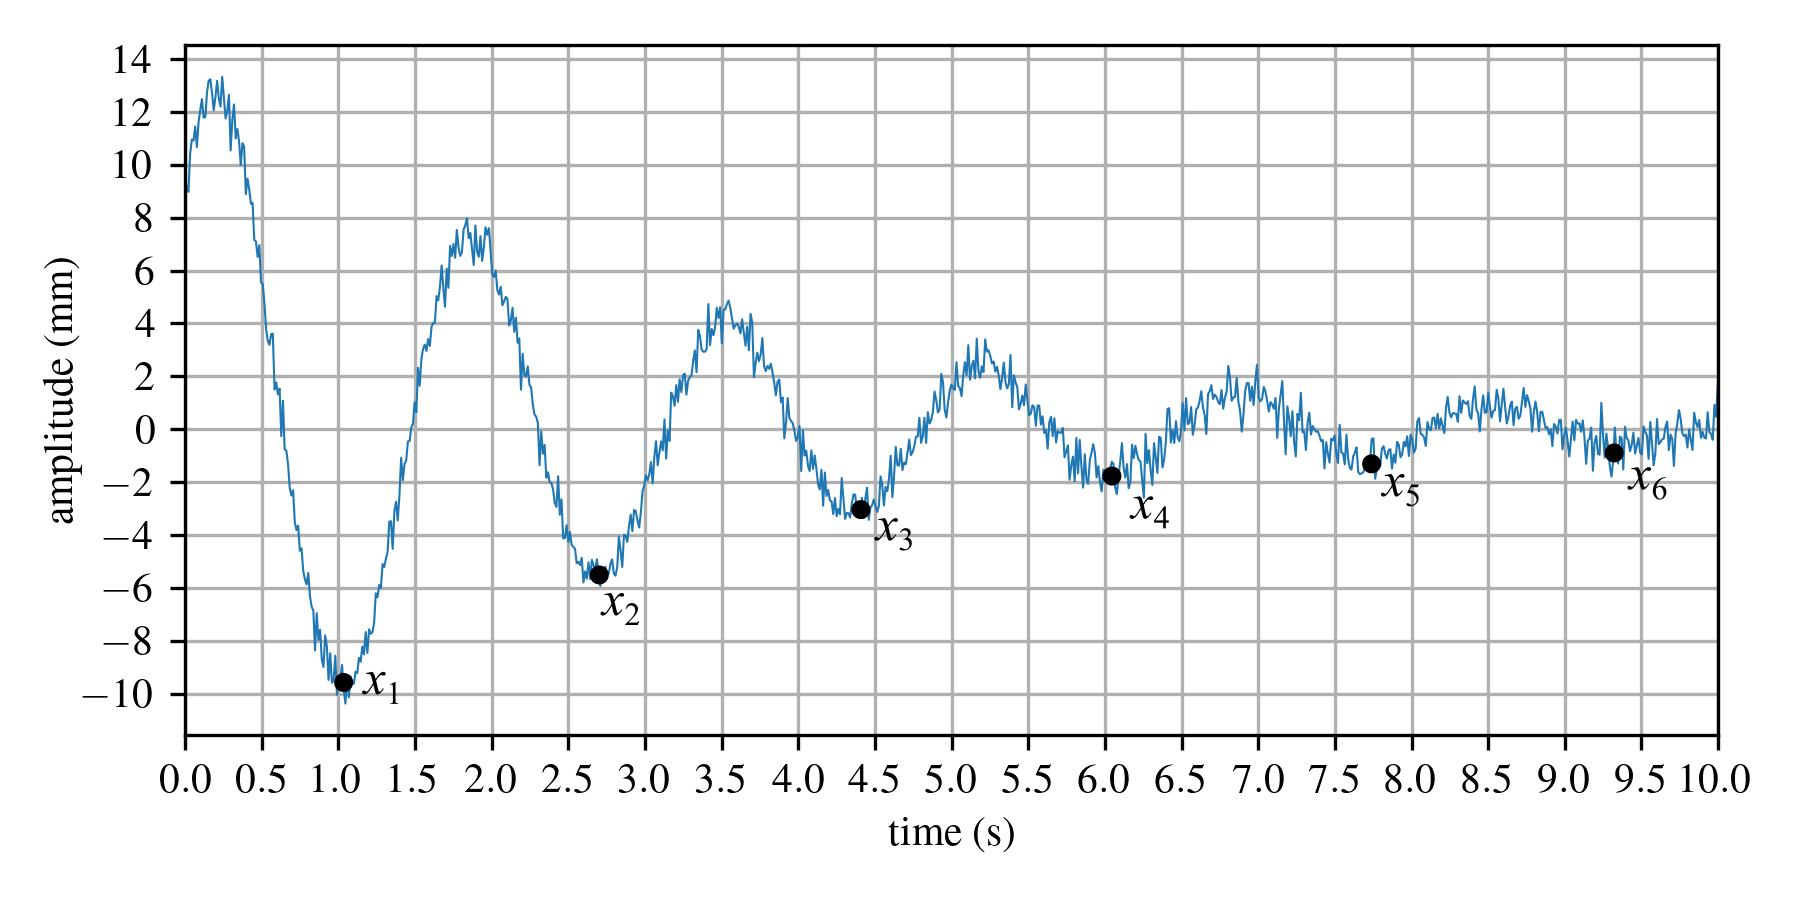
\includegraphics[width=1\linewidth]{../figures/Logarithmic_decrement_with_noise.png}
				\caption{Response from an experimental system with noise.}
				\label{fig:Logarithmic_decrement_with_noise}
			\end{figure}
			
			\noindent\textbf{Solution:} 
						
			First, from the plot we can determine that $x_1=-9.5$ mm and $x_4=-1.8$ mm where $n=3$. Thereafter, we can solve for $\delta$:  
			\begin{equation}
				\delta = \frac{1}{3}\text{ln}\bigg(\frac{x_{\text{1}}}{x_{\text{4}}}\bigg) = \frac{1}{3}\text{ln}\bigg(\frac{-9.5}{-1.8}\bigg) = 0.554
			\end{equation}						
			Next, we can calculate $\zeta$, as: 
			\begin{equation}
				\zeta = \frac{\delta}{\sqrt{4\pi^2+\delta^2}} = \frac{0.554}{\sqrt{4\pi^2+0.554^2}} = 0.0879
			\end{equation}
			And lastly:			
			\begin{equation}
				c = \zeta 2\sqrt{km} = 0.0879 \cdot 2\sqrt{43 \cdot 3} = 2.0 \text{ kg/s}
			\end{equation}	

\end{example}

	
\begin{example}

			A vehicle wheel, tire, and suspension can be modeled as a SDOF spring and mass as depicted below: %The mass of the wheel and tire is measured to be 300 kg and its frequency of oscillation is observed to be 10 rad/sec. What is the stiffness of the wheel assembly?
			
			\begin{figure}[H]
				\centering
				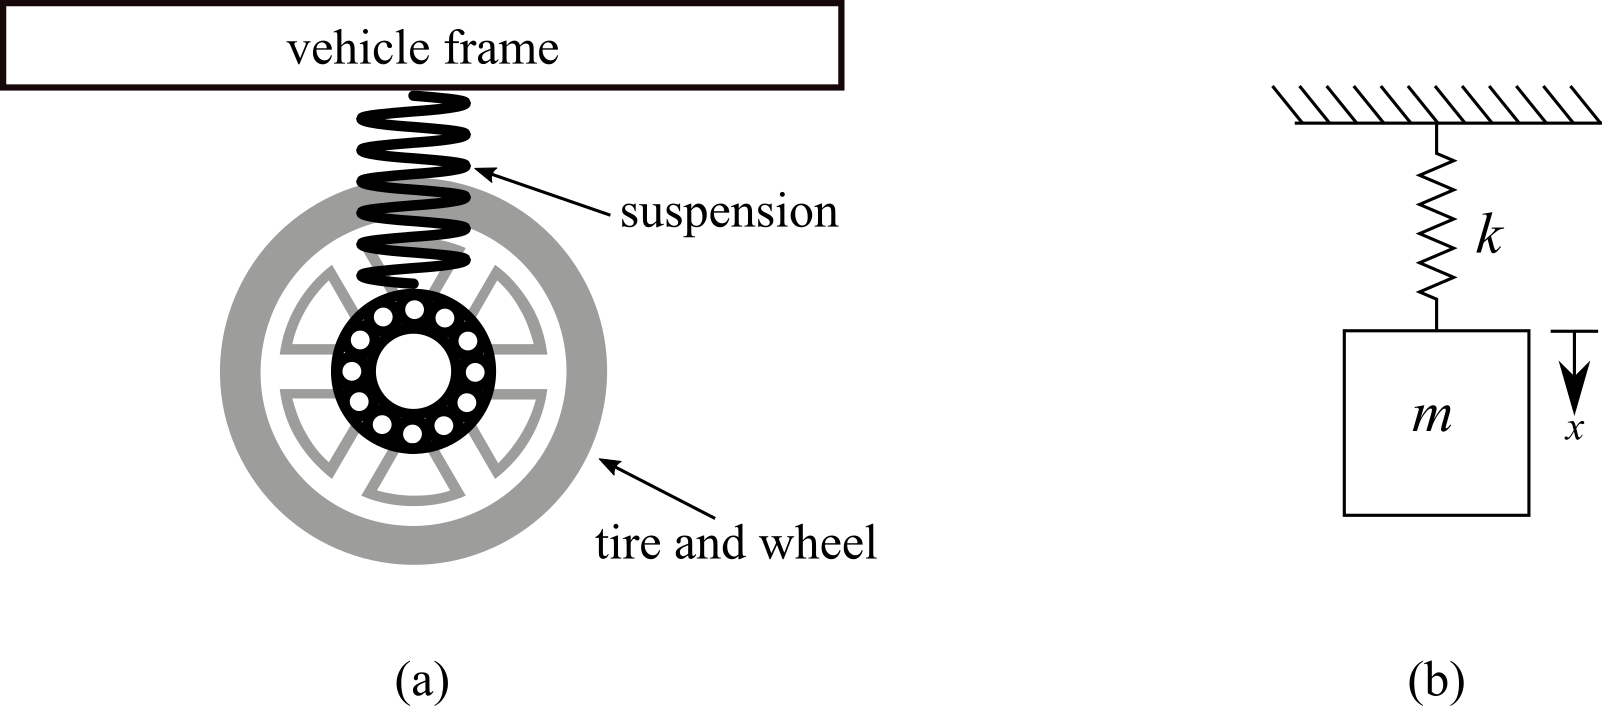
\includegraphics[width=1\linewidth]{../figures/Vehicle_wheel_undamped.png}
				\caption{Modeling of a vehicle wheel, tire, and suspension showing: (a) Graphical representation; and (b) a spring-mass model.}
				\label{fig:vehicle_wheel_undamped}
			\end{figure}	
			
			The free response of a 1000-kg automobile with a stiffness of $k$ = 400,000 N/m is observed to be underdamped. Modeling the automobile as a single-degree-of-freedom oscillation in the vertical direction, as annotated in figure \ref{fig:vehicle_wheel_undamped}, determine the damping coefficient if the displacement at $t_1$ is measured to be 2 cm and 0.22 cm at $t_2$.

			\noindent\textbf{Solution:} 
						
			Knowing $x_1$ = 2 cm and $x_2$ = 0.22 cm and $t_2 = T + t_1$, therefore:
			\begin{equation}
				\delta = \text{ln}\frac{x_1}{x_2} = \text{ln}\frac{2}{0.22} = 2.207
			\end{equation}			
			and:
			\begin{equation}
				\zeta = \bigg(\frac{\delta}{\sqrt{4\pi^2+\delta^2}}\bigg) = \bigg(\frac{2.207}{\sqrt{4\pi^2+2.207^2}}\bigg) = 0.331
			\end{equation}
			therefore, we can obtain the damping coefficient as
			\begin{equation}
				c = 2\zeta\sqrt{km}=2(0.331)\sqrt{400,000 \cdot 1,000} = 13,256 \hspace{1ex} 
				\text{kg/s} 
			\end{equation}	

\end{example}














	\pagebreak
	\renewcommand{\thepage}{}
	\renewcommand\refname{References Cited}
	\pagestyle{plain}
	\bibliographystyle{Downey_NSF}
	\bibliography{Chapter_1_Basic_Concepts}


















\end{document}

